% This is samplepaper.tex, a sample chapter demonstrating the
% LLNCS macro package for Springer Computer Science proceedings;
% Version 2.21 of 2022/01/12
%
\documentclass[runningheads]{llncs}
% packages
\usepackage{amsmath,amssymb}
\usepackage{graphicx}
\usepackage{hyperref}

% directory of figures
\graphicspath{ {figs} }

% latin bold lower
\newcommand{\ba}{\mathbf{a}} 
\newcommand{\bc}{\mathbf{c}} 
\newcommand{\be}{\mathbf{e}} 
\newcommand{\bh}{\mathbf{h}} 
\newcommand{\bp}{\mathbf{p}} 
\newcommand{\bt}{\mathbf{t}} 
\newcommand{\bs}{\mathbf{s}} 
\newcommand{\bu}{\mathbf{u}} 
\newcommand{\bv}{\mathbf{v}} 
\newcommand{\bw}{\mathbf{w}} 
\newcommand{\bx}{\mathbf{x}} 
\newcommand{\by}{\mathbf{y}} 
\newcommand{\bz}{\mathbf{z}} 
\newcommand{\bm}{\mathbf{m}} 

% latin bold upper
\newcommand{\bA}{\mathbf{A}} 
\newcommand{\bB}{\mathbf{B}} 
\newcommand{\bC}{\mathbf{C}} 
\newcommand{\bI}{\mathbf{I}} 
\newcommand{\bJ}{\mathbf{J}} 
\newcommand{\bL}{\mathbf{L}} 
\newcommand{\bM}{\mathbf{M}} 
\newcommand{\bP}{\mathbf{P}}
\newcommand{\bQ}{\mathbf{Q}} 
\newcommand{\bR}{\mathbf{R}} 
\newcommand{\bT}{\mathbf{T}} 
\newcommand{\bU}{\mathbf{U}} 
\newcommand{\bV}{\mathbf{V}} 
\newcommand{\bW}{\mathbf{W}} 
\newcommand{\bX}{\mathbf{X}} 
\newcommand{\bY}{\mathbf{Y}} 
\newcommand{\bZ}{\mathbf{Z}} 

% latin cal upper
\newcommand{\cF}{\mathcal{F}} 
\newcommand{\cG}{\mathcal{G}} 
\newcommand{\cI}{\mathcal{I}} 
\newcommand{\cL}{\mathcal{L}} 
\newcommand{\cM}{\mathcal{M}} 
\newcommand{\cN}{\mathcal{N}} 
\newcommand{\cS}{\mathcal{S}} 
\newcommand{\cT}{\mathcal{T}} 
\newcommand{\cW}{\mathcal{W}} 
\newcommand{\cX}{\mathcal{X}} 
\newcommand{\cZ}{\mathcal{Z}} 

% latin bb upper
\newcommand{\bbE}{\mathbb{E}} 
\newcommand{\bbI}{\mathbb{I}} 
\newcommand{\bbP}{\mathbb{P}} 
\newcommand{\bbR}{\mathbb{R}}
\newcommand{\bbX}{\mathbb{X}} 
\newcommand{\bbY}{\mathbb{Y}}
\newcommand{\bbW}{\mathbb{W}} 

% greek bold lower
\newcommand{\bepsilon}{\boldsymbol{\epsilon}} 
\newcommand{\btheta}{\boldsymbol{\theta}} 
\newcommand{\blambda}{\boldsymbol{\lambda}} 
\newcommand{\bpi}{\boldsymbol{\pi}} 
\newcommand{\bmu}{\boldsymbol{\mu}} 
\newcommand{\bsigma}{\boldsymbol{\sigma}} 
\newcommand{\bphi}{\boldsymbol{\phi}} 

% greek bold upper
\newcommand{\bSigma}{\boldsymbol{\Sigma}} 

\DeclareMathOperator*{\argmin}{arg\,min}
\DeclareMathOperator*{\argmax}{arg\,max}

% transpose
\newcommand{\T}{^{\text{\tiny\sffamily\upshape\mdseries T}}}
%
\usepackage[T1]{fontenc}
% T1 fonts will be used to generate the final print and online PDFs,
% so please use T1 fonts in your manuscript whenever possible.
% Other font encondings may result in incorrect characters.
%
\usepackage{graphicx}
% Used for displaying a sample figure. If possible, figure files should
% be included in EPS format.
%
% If you use the hyperref package, please uncomment the following two lines
% to display URLs in blue roman font according to Springer's eBook style:
\usepackage{color}
\renewcommand\UrlFont{\color{blue}\rmfamily}
\urlstyle{rm}
%
\begin{document}
%
\title{Sample Size Determination:\\Likelihood Bootstrapping}
%
\titlerunning{Sample Size Determination: Likelihood Bootstrapping}
% If the paper title is too long for the running head, you can set
% an abbreviated paper title here
%
%\author{Nikita Kiselev\inst{1} \and Andrey Grabovoy\inst{1}}
\author{Nikita Kiselev\inst{1} \and Andrey Grabovoy\inst{2}}
%
\authorrunning{N. Kiselev, A. Grabovoy}
% First names are abbreviated in the running head.
% If there are more than two authors, 'et al.' is used.
%
\institute{Moscow Institute of Physics and Technology, Moscow, Russia;\\
$^1$\texttt{kiselev.ns@phystech.edu};\\
$^2$\texttt{grabovoy.av@phystech.edu}.
}
%
\maketitle % typeset the header of the contribution
%
\begin{abstract}
The problem of determining an appropriate sample size is essential for constructing an efficient machine learning model. However, current techniques are either not rigorously proven or are specific to a particular statistical hypothesis regarding the distribution of model parameters. In this paper we propose two methods based on the likelihood values on resampled subsets. We demonstrate the validity of one of these methods in a linear regression model. Computational experiments show the convergence of the proposed functions as the sample size increases.

\keywords{Sufficient sample size \and Likelihood bootstrapping \and Linear regression}
\end{abstract}
%
%
%
\section{Introduction}
The process of supervised machine learning entails the selection of a predictive model from a family of parametric models, a decision often based on specific statistical assumptions, such as optimizing a particular quality function. A model that aligns with these statistical assumptions is termed as a \textit{adequate} model \cite{bies2006genetic,cawley2010over}.

In the planning phase of a computational experiment, it is crucial to estimate the minimum required sample size, which refers to the number of objects necessary to construct a suitable model. The sample size needed to develop an adequate predictive model is called \textit{sufficient} \cite{byrd2012sample,figueroa2012predicting,balki2019sample}. 

This study focuses on the determination of a sufficient sample size, a topic that has been extensively researched with methods categorized into statistical, Bayesian, and heuristic approaches.

Early investigations on this subject, such as \cite{Adcock1988,Joseph1995}, establish a specific statistical criterion, where the sample size estimation method associated with this criterion guarantees achieving a fixed statistical power with a Type I error not exceeding a specified value. Statistical methods include the Lagrange multipliers test \cite{self1988power}, the Likelihood ratio test \cite{shieh2000power}, the Wald statistic \cite{shieh2005power}. Statistical methods have certain limitations associated with their practical application. They enable the estimation of the sample size based on assumptions about data distribution and information regarding the consistency of observed values with the assumptions of the null hypothesis.

The Bayesian method is another approach to this problem. In the study \cite{Lindley1997}, the sufficient sample size is ascertained by maximizing the expected utility function, which may explicitly incorporate parameter distribution functions and penalties for increasing the sample size. This study also explores alternative methods based on restricting a certain quality criterion for model parameter estimation. Notable among these criteria are the Average Posterior Variance Criterion (APVC), Average Coverage Criterion (ACC), Average Length Criterion (ALC), and Effective Sample Size Criterion (ESC). These criteria have been further refined in subsequent research, such as \cite{PhamGia1997} and \cite{Gelfand2002}. Eventually, the authors of \cite{Cao2009} conducted a theoretical and practical comparison of methods from \cite{Adcock1988,Joseph1995,Lindley1997}.

Researchers like \cite{Brutti2014} and \cite{Pezeshk2008} delve into the distinctions between Bayesian and frequentist approaches in determining sample size, proposing robust methods for the Bayesian approach and providing illustrative examples for certain probabilistic models.

The paper \cite{Grabovoy2022} examines various methods for sample size estimation in generalized linear models, encompassing statistical, heuristic, and Bayesian methods. Techniques such as Lagrange Multiplier Test, Likelihood Ratio Test, Wald Test, Cross-Validation, Bootstrap, Kullback-Leibler Criterion, Average Posterior Variance Criterion, Average Coverage Criterion, Average Length Criterion, and Utility Maximization are analyzed. The authors highlight the potential of combining Bayesian and statistical approaches to estimate sample size when available sample sizes are insufficient.

In \cite{MOTRENKO2014743}, a method for determining sample size in logistic regression is presented, utilizing cross-validation and Kullback-Leibler divergence between posterior distributions of model parameters on similar subsamples. Similar subsamples refer to those that can be derived from each other by adding, removing, or replacing one object.

%The genetic algorithm, as described in \cite{Goldberg1988}, can be employed to approximate a given set of functions. This algorithm represents an optimization process where a population of candidates (known as individuals) evolves towards superior solutions \cite{Mirjalili2019}. Each individual possesses a set of characteristics (genes or phenotypes) that can evolve over time. Evolution occurs through crossover or mutation operations. The evolution commences with a random population, with each generation serving as the foundation for the next one. The fitness of individuals is assessed in each generation, and individuals with superior fitness are chosen to create a new generation \cite{Kramer2017}. The algorithm concludes after reaching the maximum number of generations or achieving satisfactory results, resulting in each new generation becoming more adapted to the environment.

This paper discusses several approaches to determining a sufficient sample size. It is proposed to estimate the mathematical expectation and variance of the likelihood function on bootstrapped subsamples. A small change in these values when adding another object indicates that a sufficient number of objects in the sample has been reached. The correctness of the definition in the linear regression model is proved. The presented method is easy to use in practice. To do this, it is proposed to calculate the value of the loss function instead of the likelihood. 
%The paper also proposes a method that allows you to estimate a sufficient sample size if there are not enough objects. A genetic algorithm is used to approximate a large number of dependencies of the error function on the sample size on open datasets with regression and classification tasks.

\section{Problem statement}
An object is defined as a pair $(\mathbf{x}, y)$, where $\mathbf{x} \in \mathbb{X} \subseteq \mathbb{R}^n$ is the feature vector, and $y \in \mathbb{Y}$ is the target variable. In regression problems $\mathbb{Y} = \mathbb{R}$, and in $K$-class classification problems $\mathbb{Y} = \{1, \ldots, K\}$.

The feature-object matrix for a sample $\mathfrak{D}_m = \left\{ (\mathbf{x}_i, y_i) \right\}, i \in \mathcal{I} = \{ 1, \ldots, m \}$ of size $m$ is called the matrix $\mathbf{X}_m = \left[ \mathbf{x}_1, \ldots, \mathbf{x}_m \right]^{\top} \in \mathbb{R}^{m \times n}$.

The target variable vector for a sample $\mathfrak{D}_m = \left\{ (\mathbf{x}_i, y_i) \right\}, i \in \mathcal{I} = \{ 1, \ldots, m \}$ of size $m$ is denoted by $\mathbf{y}_m = \left[ y_1, \ldots, y_m \right]^{\top} \in \mathbb{Y}^m$.

A model is a parametric family of functions $f$, mapping the Cartesian product of the set of feature vector values $\mathbb{X}$ and the set of parameter values $\mathbb{W}$ to the set of target variable values $\mathbb{Y}$: 
\[ f: \mathbb{X} \times \mathbb{W} \to \mathbb{Y}. \]

A probabilistic model is a joint distribution
\[ p(y, \mathbf{w} | \mathbf{x}) = p(y | \mathbf{x}, \mathbf{w}) p(\mathbf{w}): \mathbb{Y} \times \mathbb{W} \times \mathbb{X} \to \mathbb{R}^+, \]
where $\mathbf{w} \in \mathbb{W}$ is the set of model parameters, $p(y | \mathbf{x}, \mathbf{w})$ specifies the likelihood of an object, and $p(\mathbf{w})$ represents the prior distribution of parameters.

The likelihood function of a sample $\mathfrak{D}_m = \left\{ (\mathbf{x}_i, y_i) \right\}, i \in \mathcal{I} = \{ 1, \ldots, m \}$ of size $m$, where $\mathbf{x}_1, \ldots, \mathbf{x}_m$ are i.i.d. together, is defined as 
\[ L(\mathfrak{D}_m, \mathbf{w}) = p(\mathbf{y}_m | \mathbf{X}_m, \mathbf{w}) = \prod_{i=1}^{m} p(y_i | \mathbf{x}_i, \mathbf{w}). \]
Its logarithm
\[ l(\mathfrak{D}_m, \mathbf{w}) = \sum\limits_{i=1}^{m} \log p(y_i | \mathbf{x}_i, \mathbf{w}) \]
is called the logarithmic likelihood function. Unless stated otherwise, we consider samples to be i.i.d.

The maximum likelihood estimate of a set of parameters $\mathbf{w} \in \mathbb{W}$ based on the subsample $\mathfrak{D}_k$ of size $k$ is given by 
\[ \hat{\mathbf{w}}_{k} = \arg\max_{\mathbf{w} \in \mathbb{W}} L(\mathfrak{D}_k, \mathbf{w}). \]

The task is to determine the sufficient sample size $m^*$. Let a criterion $T$ be given. E.g. it can be constructed based on heuristics regarding the behaviour of model parameters.
\begin{definition}
    The sample size $m^*$ is called \textbf{sufficient} according to the criterion $T$, if $T$ holds for all $k \geqslant m^*$.
\end{definition}

\section{Proposed sample size determination methods}

In this section, we will assume that $m^*\leqslant m$ is valid. This means that we just need to formalize which sample size can be considered sufficient. To determine sufficiency, we will use the likelihood function. When there are enough objects available, it is quite natural to expect that the resulting parameter estimate will not change much from one sample realization to another \cite{Joseph1997,Joseph1995}. The same can be said about the likelihood function. Thus, we formulate which sample size can be considered sufficient.

\begin{definition}
    \label{sufficient-variance}
    Let's fix some positive number $\varepsilon > 0$. The sample size $m^*$ is called \textbf{D-sufficient} if for all $k\geqslant m^*$
    \[ D(k) = \mathbb{D}_{\hat{\mathbf{w}}_{k}} L(\mathfrak{D}_m, \hat{\mathbf{w}}_{k}) \leqslant \varepsilon. \]
\end{definition}

On the other hand, when there are enough objects available, it is also quite natural that when adding another object to consideration, the resulting parameter estimate will not change much. Let's formulate another definition.

\begin{definition}
    \label{sufficient-difference}
    Let's fix some positive number $\varepsilon > 0$. The sample size $m^*$ is called \textbf{M-sufficient} if for all $k\geqslant m^*$ 
    \[ M(k) = \left| \mathbb{E}_{\hat{\mathbf{w}}_{k+1}} L(\mathfrak{D}_m, \hat{\mathbf{w}}_{k+1}) - \mathbb{E}_{\hat{\mathbf{w}}_{k}} L(\mathfrak{D}_m, \hat{\mathbf{w}}_{k}) \right| \leqslant \varepsilon. \]
\end{definition}
In the definitions above instead of the likelihood function $L(\mathfrak{D}_m, \hat{\mathbf{w}}_{k})$ we can consider its logarithm $l(\mathfrak{D}_m, \hat{\mathbf{w}}_{k})$.

Suppose that $\mathbb{W} = \mathbb{R}^n$. Recall that the Fisher information is called the matrix
\[ \left[\mathcal{I}(\mathbf{w})\right]_{ij} = - \mathbb{E}\left[ \dfrac{\partial^2 \log p(\mathbf{y} | \mathbf{x}, \mathbf{w})}{\partial w_i \partial w_j} \right]. \]
A known result is the asymptotic normality of the maximum likelihood estimate, that is, $\sqrt{k}\left(\hat{\mathbf{w}}_k -\mathbf{w}\right)\xrightarrow{d}\mathcal{N}\left(0, \mathcal{I}^{-1}(\mathbf{w})\right)$. Convergence in the distribution generally does not imply convergence of the moments of a random vector. Nevertheless, if we assume the latter, then in some models it is possible to prove the correctness of our proposed definition of M-sufficient sample size.

For convenience, we denote the distribution parameters $\hat{\mathbf{w}}_k$ as follows: mathematical expectation $\mathbb{E}\hat{\mathbf{w}}_k=\mathbf{m}_k$ and the covariance matrix $\mathbb{D} \hat{\mathbf{w}}_k = \mathbf{\Sigma}_k$. Then the following theorem holds, the proof of which is given in the appendix.

\begin{theorem}\label{theorem}
    Let $\|\mathbf{m}_{k+1} - \mathbf{m}_k\|_2 \to 0$ and $\|\mathbf{\Sigma}_{k+1} - \mathbf{\Sigma}_k\|_{F}\to 0$ as $k\to \infty$. Then, in the linear regression model, the definition of M-sufficient sample size is correct. Namely, for any $\varepsilon > 0$, there is such a $m^*$ that for all $k\geqslant m^*$ $M(k)\leqslant\varepsilon$ is satisfied.
\end{theorem}

\begin{corollary}\label{corollary}
    Let $\|\mathbf{m}_k - \mathbf{w}\|_2\to 0$ and $\|\mathbf{\Sigma}_k - \left[k\mathcal{I}(\mathbf{w})\right]^{-1}\|_{F}\to 0$ for $k \to \infty$. Then, in the linear regression model, the definition of an M-sufficient sample size is correct. 
\end{corollary}

By condition, one sample is given. Therefore, in the experiment it is not possible to calculate the mathematical expectation and variance specified in the definitions. To evaluate them, we will use the bootstrap technique. Namely, we will generate from the given $\mathfrak{D}_m$ a number of $B$ subsamples of size $k$ with a return. For each of them, we get an estimate of the parameters $\hat{\mathbf{w}}_{k}$ and calculate the value of $L(\mathfrak{D}_m, \hat{\mathbf{w}}_{k})$. For the estimation, we will use a sample mean and an unbiased sample variance (for bootstrap samples).

The definitions proposed above can also be applied in those problems where an arbitrary loss function is minimized rather than the likelihood function is maximized. We do not provide any theoretical justification for this, but in practice such a heuristic turns out to be quite successful.

\section{Computational experiment}

This section provides an empirical study of the proposed methods. Experiments were conducted on synthetic data and dataset Liver Disorders from \cite{UCI}. The code is available in open source in the GitHub repository\footnote{\href{https://github.com/kisnikser/Likelihood-Bootstrapping}{\texttt{https://github.com/kisnikser/Likelihood-Bootstrapping}}}.

Synthetic data is generated from linear regression and logistic regression models. The number of objects is 1000, the number of features is 20. $B=1000$ bootstrapped subsamples are used. The values of $D(k)$ and $M(k)$ are calculated.  Regression dataset Liver Disorders has 345 objects and 5 features. We also use $B=1000$ subsamples made by bootstrapping to estimate mean and variance of the loss function. 

In the Fig.~\ref{synthetic-regression}, we can observe the obtained dependencies between the available sample size $k$ and the proposed functions $D(k)$ and $M(k)$ for the synthetic regression dataset. Results for the synthetic classification dataset are in the Fig.~\ref{synthetic-classification}. At the same time, in the Fig.~\ref{liver-disorders}, we see the same plots for the Liver Disorders dataset. It can be seen that in all cases, the values of $D(k)$ and $M(k)$ approaches zero as the sample size increases. These empirical results confirm the theoretical ones obtained earlier.

\begin{figure}[ht]
    \centering
    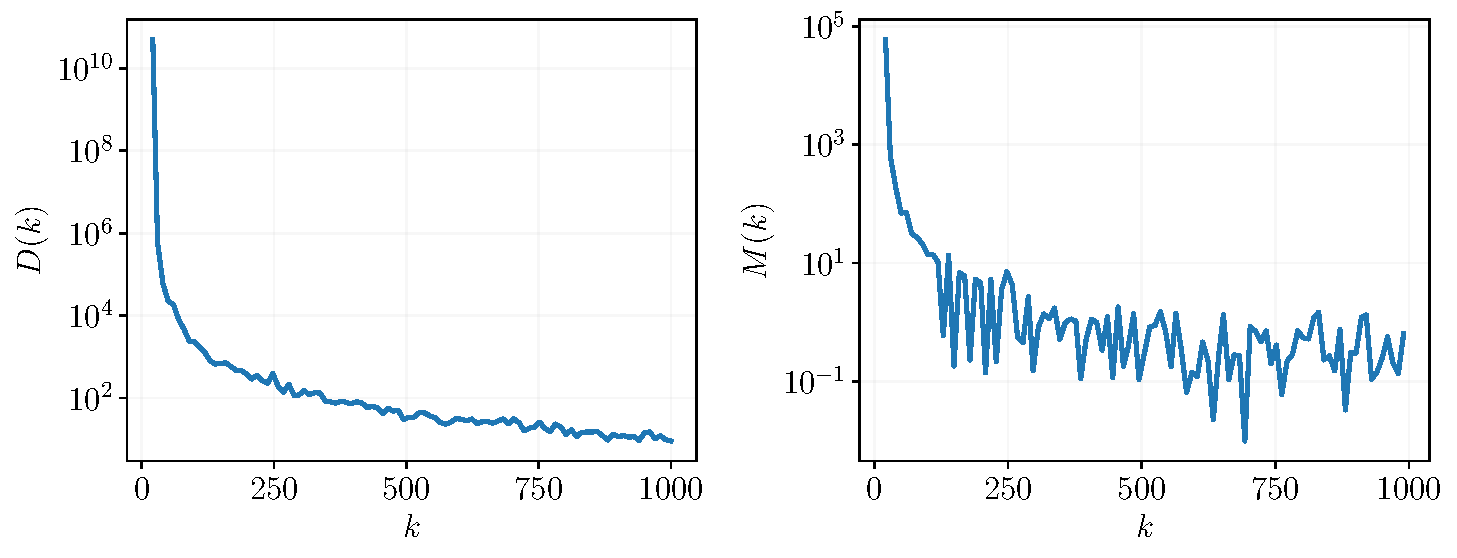
\includegraphics[width=\textwidth]{synthetic-regression}
    \caption{Convergence of the proposed functions $D(k)$ and $M(k)$ for the synthetic regression dataset, i.e. linear regression model. Both functions tends to zero as the sample size increases.}
    \label{synthetic-regression}
\end{figure}

\begin{figure}[ht]
    \centering
    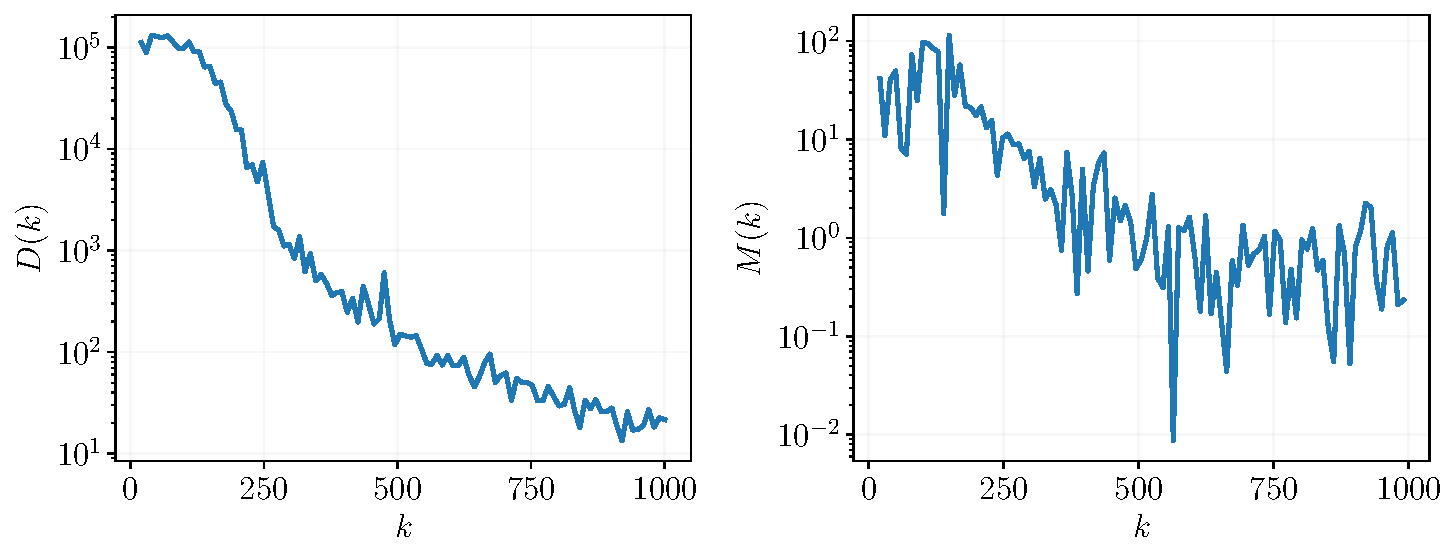
\includegraphics[width=\textwidth]{synthetic-classification}
    \caption{Convergence of the proposed functions $D(k)$ and $M(k)$ for the synthetic classification dataset, i.e. logistic regression model. Both functions tends to zero as the sample size increases.}
    \label{synthetic-classification}
\end{figure}

\begin{figure}[ht]
    \centering
    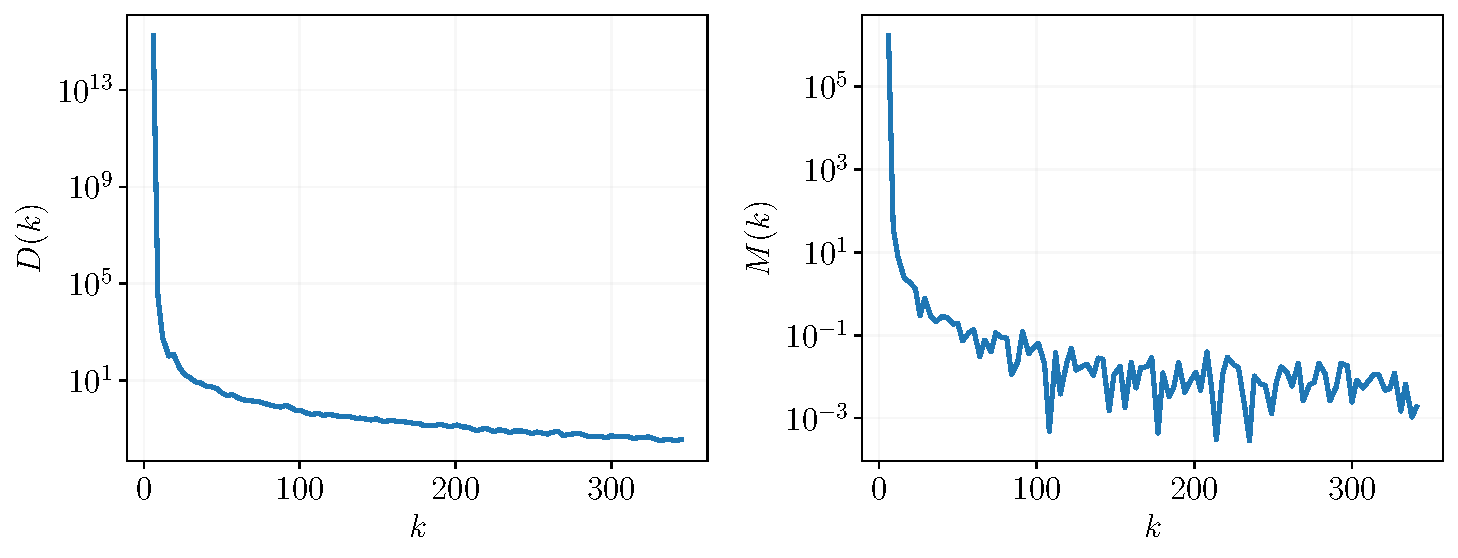
\includegraphics[width=\textwidth]{liver-disorders}
    \caption{Convergence of the proposed functions $D(k)$ and $M(k)$ for the Liver Disorders dataset. Both functions tends to zero as the sample size increases.}
    \label{liver-disorders}
\end{figure}

For the definitions of D-sufficiency and M-sufficiency, there is a hyperparameter $\varepsilon$, which corresponds to the threshold for a sufficient sample size $m^*$. In order to study the dependence between them, we introduce Fig.~\ref{sufficient-vs-threshold}, which shows what sample sizes can be chosen to provide a certain level of confidence.

\begin{figure}[ht]
    \centering
    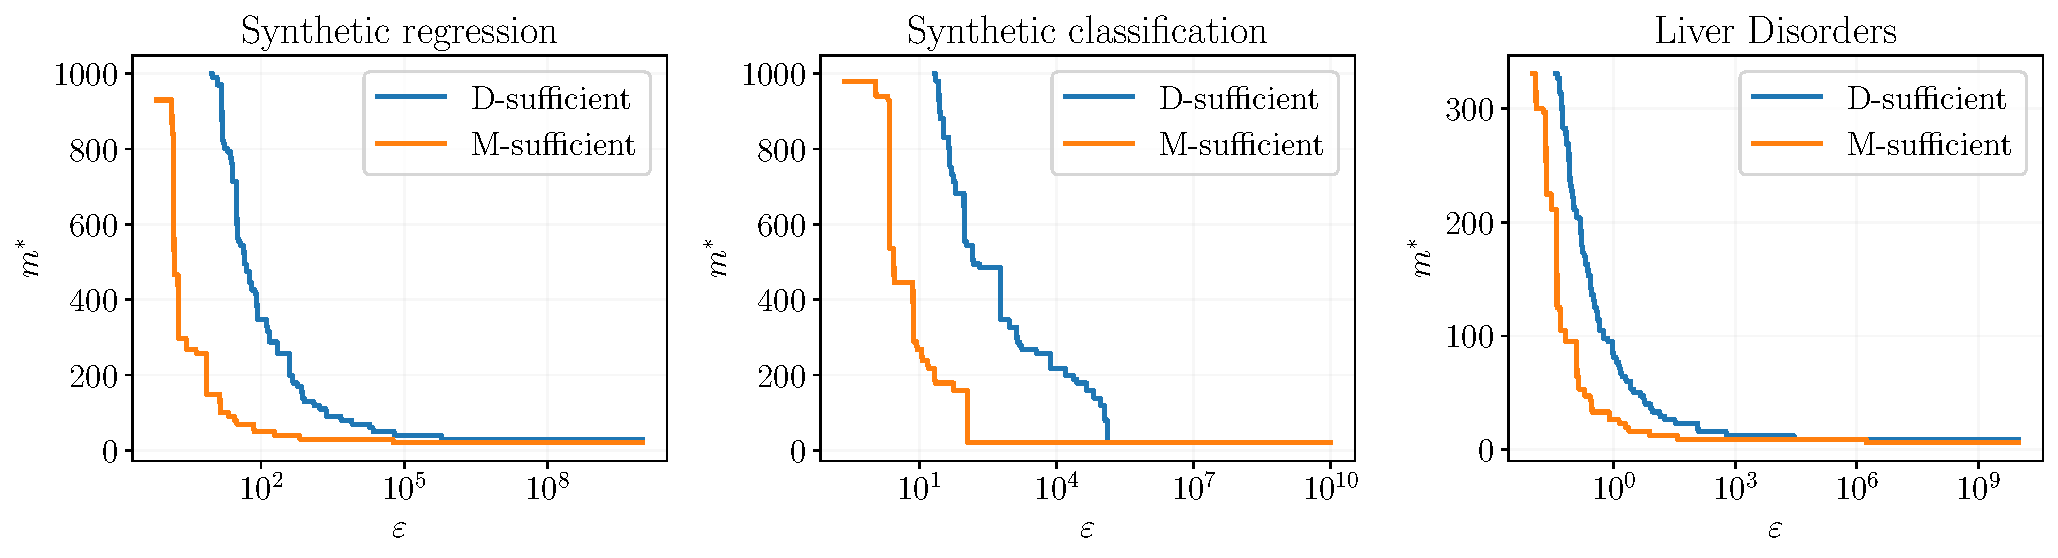
\includegraphics[width=\textwidth]{sufficient-vs-threshold}
    \caption{Sufficient sample size versus threshold for three datasets: synthetic regression, synthetic classification, and Liver Disorders. As the threshold value $\varepsilon$ increases, the sufficient sample size decreases. It means, that one can choose fewer objects to satisfy the desirable values of the proposed functions $D(k)$ and $M(k)$. }
    \label{sufficient-vs-threshold}
\end{figure}

To compare the performance of the proposed methods on different datasets, samples have been chosen from the open repository \cite{UCI}. The detailed information about each dataset, the number of observations and number of features, are provided in Table~\ref{table}. For demonstration purposes, a value of the hyperparameter $\varepsilon$ has been selected, at which the value of the target function, either $D(k)$ or $M(k)$, decreases by half. The corresponding results are in Table~\ref{table}. Omissions mean that the initial sample size is not sufficient.

\begin{table}[ht]
    \centering
    \caption{Comparison of the proposed methods of sample size determination: based on $D(k)$ and $M(k)$. For each of the proposed functions the threshold value $\varepsilon$ was chosen in such way that the initial function value decreases by half. The results were obtained for a variety of datasets with regression task. Omissions in the table mean that the initial sample size is not sufficient.}\label{table}
    \begin{tabular}{|l|c|c|c|c|}
    \hline
    Dataset name & Objects $m$ & Features $n$ & D & M \\
    \hline
    Abalone & 4177 & 8 & 96 & 96  \\
    Auto MPG & 392 & 8 & 15 & 15 \\
    Automobile & 159 & 25 & 70 & 156  \\
    Liver Disorders & 345 & 6 & 12 & 19  \\
    Servo & 167 & 4 & 41 & ---  \\
    Forest fires & 517 & 12 & 208 & --- \\
    Wine Quality & 6497 & 12 & 144 & 144  \\
    Energy Efficiency & 768 & 9 & 24 & 442  \\
    Student Performance & 649 & 32 & 129 & 177  \\
    Facebook Metrics & 495 & 18 & 31 & 388   \\
    Real Estate Valuation & 414 & 7 & 15 & 23  \\
    Heart Failure Clinical Records & 299 & 12 & 63 & 224  \\
    Bone marrow transplant: children & 142 & 36 & --- & --- \\
    \hline
    \end{tabular}
\end{table}

\clearpage
\section{Discussion}

In this paper, we have proposed two novel methods for determining a sufficient sample size based on the likelihood values on resampled subsets. The first method, referred to as D-sufficiency, relies on the variance of the likelihood function, while the second method, M-sufficiency, focuses on the difference in the expected likelihood function when adding an additional object to the sample. We have demonstrated the validity of the M-sufficient sample size definition in a linear regression model, under certain conditions on the model parameters.

The computational experiments conducted on synthetic and real-world datasets have shown that the proposed functions, $D(k)$ and $M(k)$, converge to zero as the sample size increases. The experiments also highlight the practicality of the methods, as they can be easily applied to various datasets.

The proposed methods have the potential to be applied to a wide range of models and datasets, beyond linear regression. Although we have only proved the correctness of the M-sufficient sample size definition for linear regression, the empirical results suggest that the methods may be effective for other models as well. Future work should focus on extending the theoretical analysis to other models, including probably neural networks.

\section{Conclusion}

This paper introduces two novel methods, D-sufficiency and M-sufficiency, for determining a sufficient sample size based on likelihood values on resampled subsets. The validity of the M-sufficient sample size definition is demonstrated in a linear regression model, and computational experiments on synthetic and real-world datasets show that the proposed functions converge to zero as the sample size increases, highlighting the practicality of the methods. Future work should focus on extending the theoretical analysis to other models, including neural networks.

%
% ---- Bibliography ----
%
% BibTeX users should specify bibliography style 'splncs04'.
% References will then be sorted and formatted in the correct style.
%
\clearpage
\bibliographystyle{splncs04}
\bibliography{references}
%

\clearpage
\appendix

\section{Proof of Theorem \ref{theorem}}

\begin{proof}
Consider the definition of an M-sufficient sample size in terms of the logarithm of the likelihood function. In a linear regression model
    \[ L\left( \mathfrak{D}_m, \hat{\mathbf{w}}_k \right) = p(\mathbf{y} | \mathbf{X}, \hat{\mathbf{w}}_k) = \prod_{i=1}^{m} p(y_i | \mathbf{x}_i, \hat{\mathbf{w}}_k) = \prod_{i=1}^{m} \mathcal{N}\left( y_i | \hat{\mathbf{w}}_k^{\top} \mathbf{x}_i, \sigma^2 \right) = \]
    \[= \left(2\pi\sigma^2 \right)^{-m/2} \exp\left(-\dfrac{1}{2\sigma^2}\|\mathbf{y} -\mathbf{X} \hat{\mathbf{w}}_k\|_2^2 \right). \]
Take a logarithm:
    \[ l\left( \mathfrak{D}_m, \hat{\mathbf{w}}_k \right) = \log p(\mathbf{y} | \mathbf{X}, \hat{\mathbf{w}}_k) = -\dfrac{m}{2}\log\left( 2\pi\sigma^2 \right) - \dfrac{1}{2\sigma^2} \| \mathbf{y} - \mathbf{X} \hat{\mathbf{w}}_k \|_2^2. \]
Let's take the mathematical expectation of $\mathfrak{D}_k$, given that $\mathbb{E}_{\mathfrak{D}_k}\hat{\mathbf{w}}_k=\mathbf{m}_k$ and $\text{cov}(\hat{\mathbf{w}}_k) = \mathbf{\Sigma}_k$:
    \[ \mathbb{E}_{\mathfrak{D}_k} l\left( \mathfrak{D}_m, \hat{\mathbf{w}}_k \right) = -\dfrac{m}{2}\log\left( 2\pi\sigma^2 \right) - \dfrac{1}{2\sigma^2} \Big( \| \mathbf{y} - \mathbf{X} \mathbf{m}_k \|_2^2 + \text{tr}\left( \mathbf{X}^{\top}\mathbf{X} \mathbf{\Sigma}_k \right) \Big). \]
    Let's write down an expression for the difference in mathematical expectations:
    \[ \mathbb{E}_{\mathfrak{D}_{k+1}} l(\mathfrak{D}_m, \hat{\mathbf{w}}_{k+1}) - \mathbb{E}_{\mathfrak{D}_k} l(\mathfrak{D}_m, \hat{\mathbf{w}}_{k}) = \]
    \[ = \dfrac{1}{2\sigma^2} \Big( \| \mathbf{y} - \mathbf{X} \mathbf{m}_k \|_2^2 - \| \mathbf{y} - \mathbf{X} \mathbf{m}_{k+1} \|_2^2 \Big) + \dfrac{1}{2\sigma^2} \text{tr} \Big( \mathbf{X}^{\top}\mathbf{X} \left( \mathbf{\Sigma}_k - \mathbf{\Sigma}_{k+1} \Big) \right) = \]
    \[ = \dfrac{1}{2\sigma^2} \Big( 2 \mathbf{y}^{\top} \mathbf{X} (\mathbf{m}_{k+1} - \mathbf{m}_k) + (\mathbf{m}_k - \mathbf{m}_{k+1})^{\top} \mathbf{X}^{\top}\mathbf{X} (\mathbf{m}_k + \mathbf{m}_{k+1}) \Big) + \]
    \[ + \dfrac{1}{2\sigma^2} \text{tr} \Big( \mathbf{X}^{\top}\mathbf{X} \left( \mathbf{\Sigma}_k - \mathbf{\Sigma}_{k+1} \right) \Big). \]
The value of the function $M(k)$ is a module from the above expression. Let's apply the triangle inequality for the module, and then evaluate each term.\\
We estimate the first term using the Cauchy-Schwarz inequality:
\[\big| \mathbf{y}^{\top}\mathbf{X}(\mathbf{m}_{k+1}-\mathbf{m}_k)\big| \leqslant \| \mathbf{X}^{\top}\mathbf{y} \|_2 \|\mathbf{m}_{k+1} - \mathbf{m}_k\|_2. \]
    The second term is estimated using the Cauchy-Schwarz inequality, the consistency property of the spectral matrix norm, as well as the limitation of the sequence of vectors $\mathbf{m}_k$, which follows from the presented convergence condition:
\[\big| (\mathbf{m}_k - \mathbf{m}_{k+1})^{\top} \mathbf{X}^{\top}\mathbf{X} (\mathbf{m}_k + \mathbf{m}_{k+1}) \big| \leqslant \| \mathbf{X} (\mathbf{m}_k - \mathbf{m}_{k+1}) \|_2 \| \mathbf{X} (\mathbf{m}_k + \mathbf{m}_{k+1}) \|_2 \leqslant \]
    \[ \leqslant \| \mathbf{X} \|_2^2 \| \mathbf{m}_k - \mathbf{m}_{k+1} \|_2 \| \mathbf{m}_k + \mathbf{m}_{k+1} \|_2 \leqslant C \| \mathbf{X} \|_2^2 \| \mathbf{m}_k - \mathbf{m}_{k+1} \|_2. \]
    We estimate the last term using the Holder's inequality for the Frobenius norm:
    \[ \Big| \text{tr} \Big( \mathbf{X}^{\top}\mathbf{X} \left( \mathbf{\Sigma}_k - \mathbf{\Sigma}_{k+1} \right) \Big) \Big| \leqslant \| \mathbf{X}^{\top}\mathbf{X} \|_F \| \mathbf{\Sigma}_k - \mathbf{\Sigma}_{k+1} \|_F. \]
Finally, since $\|\mathbf{m}_k - \mathbf{m}_{k+1} \|_2\to 0$ and $\|\mathbf{\Sigma}_k - \mathbf{\Sigma}_{k+1}\|_{F}\to 0$ as $k\to\infty$, then $M(k)\to 0$ as $k\to \infty$, which proves the theorem.
\end{proof}

\section{Proof of Corollary \ref{corollary}}

\begin{proof}
    From the convergence conditions given, it follows that $\|\mathbf{m}_k - \mathbf{m}_{k+1} \|_2\to 0$ and $\|\mathbf{\Sigma}_k -\mathbf{\Sigma}_{k+1}\|_{F}\to 0$ for $k\to \infty$. The application of the \ref{theorem} theorem completes the proof.
\end{proof}

\end{document}
